\documentclass{beamer}
%\documentclass[trans]{beamer} %om te printen!
%\transglitter etc: kunt ge pas zien op Full Screen (Ctrl+L)
\usepackage{etex}
\usepackage{tikz}

\usepackage{graphicx,multicol}

\usepackage[all]{xy}
\usepackage{enumerate}

\usepackage{graphicx}
\usepackage{beamerouterthememiniframes, beamercolorthemeann,srcltx,hyperref}
\usepackage{amsmath,amsthm,amssymb}

\newcommand{\upuparrow}{\mathrel{\reflectbox{\rotatebox[origin=c]{90}{$\twoheadrightarrow$}}}}
\newcommand{\downdownarrow}{\mathrel{\reflectbox{\rotatebox[origin=c]{90}{$\twoheadleftarrow$}}}}
\setbeamercolor{normal text}{fg=black!70}
\setbeamertemplate{navigation symbols}{}%geen navigatie
\setbeamertemplate{blocks}[rounded][shadow=true]

%\setbeamercovered{dynamic} %te komen items in lichtgrijs
%\setbeamercolor{background canvas}{bg=black!0}%is wit

\logo{\vspace{-0.2cm}\\
\hfill
\includegraphics[height=3cm]{VUB_schild}}
%plaatst het logo op elke slide onderaan

\newcommand{\Z}{\mathbb{Z}}
\newcommand{\Q}{\mathbb{Q}}
\renewcommand{\P}{\mathbb{P}}
\newcommand{\R}{\mathbb{R}}
\newcommand{\N}{\mathbb{N}}
\newcommand{\C}{\mathbb{C}}
\newcommand{\U}{\mathcal{U}}
\newcommand{\E}{\mathbb{E}}
\newcommand{\z}{\mathcal{Z}}
\newtheorem{remark1}{Remark}
\newcommand{\LFP}{\text{LFP}}
%\columnsep=1.8cm %\columnseprule=.4pt
\newcommand{\cost}{\text{cost}}
\newcommand{\Nash}{\text{Nash}}
\newcommand{\nash}{\text{nash}}
\newcommand{\opt}{\text{opt}}
\newcommand{\copt}{\cost(a_{\opt})}
\title{Similarity on Graphs \& Hypergraphs}
\author{Filip Moons\\2$^{\text{th}}$ Master of Mathematics - Option: Education\\Promotor: Prof. Dr. P. Cara\\Presentation Master Thesis}
\date{September 2015}

\begin{document}

\begin{frame}[plain]

\includegraphics[width=0.4\paperwidth]{VUB_logo.jpg}
\vspace{2cm}
\titlepage
\end{frame}


%\section[Overzicht]{}%rechte haken dienen om niet in de outline te komen
%maar wel vanboven in het donkergroene balkje

%\begin{frame}[plain]{Outline}
%\end{frame}
%
%\begin{frame}[plain]{Outline}
%\tableofcontents[pausesections]
%\end{frame}
%
%
%\section{blabla}
%
%\begin{frame}
%\begin{alertblock}{}
%\begin{center}
%blabla
%\end{center}
%\end{alertblock}
%\end{frame}

\begin{frame}{Content}
\begin{itemize}
  \item Similarity on graphs
    \begin{itemize}
        \item HITS-algorithm
        \item Node similarity
        \item Node-edge similarity
        \item Colored graphs
    \end{itemize}
  \item Similarity on hypergraphs
    \begin{itemize}
        \item Node similarity with the incidence graph
        \item Node-edge similarity with the incidence matrix
    \end{itemize}

\end{itemize}

\end{frame}


\section{Similarity on graphs}
\subsection{HITS-algorithm}
\begin{frame}{HITS-algorithm}
\begin{block}{Idea}
\begin{figure}
  \centering
  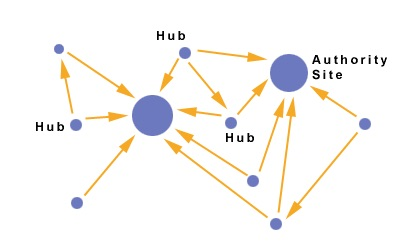
\includegraphics[scale=0.5]{hitsq.jpg}\\
\end{figure}
\end{block}

\end{frame}


\begin{frame}{HITS-algorithm}

\begin{block}{Mutually reinforcing relation}
$$\begin{cases} h_j := \sum_{i:(v_j,v_i)\in \to} a_i,\\ 
a_j := \sum_{i:(v_i,v_j)\in \to} h_i.
\end{cases}$$ 
\end{block}

\begin{block}{In matrix form}
$$\begin{pmatrix} 
\textbf{h}\\
\textbf{a}
\end{pmatrix}^{(k+1)} = \begin{pmatrix} 
0 & B\\
B^T & 0
\end{pmatrix} \begin{pmatrix} 
\textbf{h}\\
\textbf{a}
\end{pmatrix}^{(k)},\quad k = 0, 1,\ldots,$$
In compact form, we denote
\begin{eqnarray}\label{compactform}
  \mathbf{x}^{(k+1)} = M\mathbf{x}^{(k)},\quad k = 0, 1,\ldots,
\end{eqnarray}

\end{block}
\end{frame}
%\begin{frame}
%\begin{block}{}
%\begin{center}
%Introductie
%\end{center}
%\end{block}
%\end{frame}
\subsection{Node similarity}

\begin{frame}{Node similarity}


\begin{block}{Idea}
  See 
\begin{center}
\begin{tikzpicture}
           \tikzstyle{every node}=[draw,circle,fill=black,minimum size=4pt,
                            inner sep=0pt]


  \node[main node] (1) [label=left:\emph{hub}] {};
  \node[main node] (3) [label=right:\emph{authority}][right of=1] {};

  \path[every node/.style={font=\sffamily\small}]
   
    (1) edge node [left] {} (3)
  
    
\end{tikzpicture}
\end{center}
as a \textbf{structure graph} that can be replaced by any other graph.
\end{block}


\end{frame}
\section{Bibliography}
\begin{frame}
\begin{block}{}
\begin{thebibliography}{99}
\bibitem[EVES]{0} H. Eves, \emph{Elementary Matrix Theory}, Dover Publications, 
2012.
\bibitem[BAPAT] {90}R. B. Bapat, T.E.. Raghavan, \emph{Nonnegative Matrices and 
Applications}, Encyclopedia of Mathematics and its Applications 64, Cambridge University Press, 1997. 
\bibitem[STERN2010]{1} S. Sternberg, \emph{The Perron-Frobenius theorem}, Chapter 9 in Dynamical Systems, Dover Publications, 2010.
\bibitem[NOUT2008]{2} D. Noutsos, \emph{Perron-Frobenius theory and some extensions} (lecture notes), Department of Mathematics, University of Ioannina, May 2008.
\bibitem[TROPP]{tropp} J. A. Tropp, \emph{Introduction to Numerical Methods}, California Institute of 
Technology, 2005.
\bibitem[CAENEPEEL]{caenepeel} S. Caenepeel, \emph{Analyse I}, Vrije Universiteit Brussel, 2011.

 \end{block}
\end{frame}
\begin{frame}
\begin{block}{}

\bibitem[VARGA] R. S. Varga, \emph{Matrix Iterative Analysis}, Prentice-Hall, 1962. 
\bibitem[BRUALDI] R. A. Brualdi, H. J. Ryser, \emph{Combinatorial Matrix Theory}, Cambridge University 
Press, 1991
\bibitem[LANCASTER] P. Lancaster, M. Tismenetsky, \emph{The Theory of Matrices: With 
Applications}, Academic Press, 1985
\bibitem[MORROW] J. Morrow, \emph{Advanced Calculus}, University of Washington, 
2013.
\bibitem[MEU2011]{11} W. De Meuter, \emph{Algoritmen en Datastructuren I}, Vrije Universiteit Brussel, 2011.
\bibitem[KIEBOOM2011]{kieboom} R. Kieboom, \emph{Aanvulling Lineaire Algebra}, Vrije Universiteit Brussel, 2011.

\end{block}
\end{frame}
\begin{frame}
\begin{block}{}

\bibitem[ADHEMAR]{numeriekwiskunde} A. Bultheel, \emph{Inleiding tot de numerieke wiskunde}, Acco, 
2006.
\bibitem[BIN1977]{12} K.G. Binmore, \emph{Mathematical Analysis: A Straightforward Approach}, Cambridge Universitiy Press, 1977.
\bibitem[GOLUB]{golub} G. Golub, C.F. Van Loan, \emph{Matrix Computations}, 
Johns Hopkins University Press, 1996.
\bibitem[CARA]{cara} P. Cara, \emph{Discrete Wiskunde}, Vrije Universiteit Brussel - Dienst 
Uitgaven, 2011
\bibitem[LIFSHITS]{Lifshits} Y. Lifshits, \emph{Four Results of Jon Kleinberg: A Talk for St. Petersburg Mathematical 
Society}, Steklov Insitute of Mathematics at St. Petersburg, 2007.
\bibitem[PAGE]{page} S. Brin, L. Page, \emph{The Anatomy of a Large-Scale Hypertextual Web Search Engine}, Seventh International World-Wide Web Conference, 1998.
\bibitem[BLONDEL]{blondel} V. D Blondel, A. Gajardo, M. Heymans, P. Senellart, P. Van Dooren, 
\emph{A Measure of Similarity between Graph Vertices: Applications to Synonym Extraction and Web 
Searching}, Society for Industrial and Applied Mathematics, 2004.


\end{block}
\end{frame}
\begin{frame}
\begin{block}{}

\bibitem[KLEINBERG]{kleinberg} J. M. Kleinberg, \emph{Authoritative sources in a hyperlinked 
environment}, J. ACM, 1999.
\bibitem[DEIFT]{random} P. Deift, D. Gioev, \emph{Random Matrix Theory: Invariant Ensembles and 
Universality}, American Mathematical Society, January, 2009.
\bibitem[EUROVISION]{eurovision} \emph{Official website of the Eurovision Song 
Contest}, www.eurovision.tv, May, 2015.
\bibitem[SAARI]{saari} D. G. Saari,  \emph{Mathematical Structure of Voting Paradoxes: II. Positional Voting}, Journal of Economic Theory, 2000.
\bibitem[FOUC]{fouc} S. Foucart, \emph{Linear Algebra and Matrix Analysis}, 
Drexel University, 2010.
\bibitem[FRIEDL]{friedl} S. Friedl, \emph{Linear Algebra}, Rice University, 
2004.
\end{block}
\end{frame}
\begin{frame}
\begin{block}{}

\bibitem[HORN]{horn} R.A. Horn, C.R. Johnson, \emph{Matrix Analysis}, Cambridge University Press, 1985.
\bibitem[HORN2]{horn2} R.A. Horn, C.R. Johnson, \emph{Topics in Matrix 
Analysis}, Cambridge University Press, 1991.
\bibitem[TOMAS]{tomasi} C. Tomasi, \emph{Orthogonal Matrices and the Singular Value 
Decomposition}, Duke University, 2013.
\bibitem[ZAGER2003]{thesisjek} L. Zager, \emph{Graph Similarity and Matching}, 
Massachusetts Institute of Technology, 2005.
\bibitem[LAUB]{laub} Alan J. Laub, \emph{Matrix Analysis for Scientists and 
Engineers}, Siam, 2004.
    \end{block}
\end{frame}
\begin{frame}
\begin{block}{}

\bibitem[DEVOS]{devos} Matt Devos, \emph{Semidefinite Programming}, Simon Fraser 
University, 2009.
\bibitem[COLEB]{colebunders} E. Colebunders, \emph{Topologie}, Vrije 
Universiteit Brussel, 2012.
\bibitem[ZAGER]{zager} L. A.Zager, George C. Verghese, \emph{Graph similarity scoring and matching}, Applied Mathematics Letters, January, 2007.i
Analysis}, Cambridge University Press, 1991.
\bibitem[VANDOREN]{vandoren} P. Van Doren, C. Fraikin, \emph{Similarity matrices for colored 
graphs}, Bulletin of the Belgian Mathematical Society Simon Stevin, 2009.
\bibitem[BERGE]{berge} C. Berge, \textit{Graphs and Hypergraphs}, University of 
Paris (North-Holland Publishing Company), 1970.

\end{block}
\end{frame}
\begin{frame}
\begin{block}{}

\bibitem[PEARSON]{hypper}K. J. Pearson, T Zhang, \textit{On spectral hypergraph theory of the adjacency 
tensor}, Journal on Graphs and Combinatorics, Springer, 2014.
\bibitem[GALLO]{gallo} G. Gallo, G. Longo, S. Nguyen, S. Pallottino, \emph{Directed hypergraphs and 
appplications}, Journal of Discrete Applied Mathematics, Elsevier, 1997.
 
\end{block}
\end{frame}
   \end{thebibliography}
\end{document}
